\documentclass{standalone}
\usepackage{tikz}
\usepackage{ctex,siunitx,ninecolors}
\setCJKmainfont{Noto Serif CJK SC}
\usepackage{tkz-euclide}
\usepackage{amsmath}
\usepackage{wasysym}
\usetikzlibrary{patterns,calc}
\usetikzlibrary {decorations.pathmorphing, decorations.pathreplacing, decorations.shapes}
\begin{document}
\small
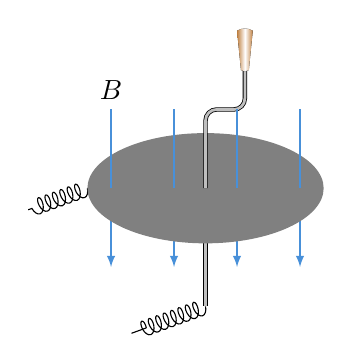
\begin{tikzpicture}[>=latex,scale=1.0]
  \draw[double=lightgray,double distance=1pt,line width=0.1mm](0,0)--(0,-1.5);
  \draw[decorate,decoration={coil,segment length=1mm,amplitude=1mm}](0,-1.5)--++(-160:0.8)(-1.5,0)--++(-160:0.8);
  \foreach \x in {-1.2,-0.4,0.4,1.2}{\draw[->,azure6](\x,0)--++(0,-1.0);}
  \fill[gray](0,0)ellipse(1.5 and 0.7);
  \draw[double=lightgray,double distance=1pt,line width=0.1mm,rounded corners](0,0)--(0,1.0)--(0.5,1)--(0.5,1.5);
  \fill[left color=brown,right color=brown,middle color=white](0.45,1.5)to[bend right](0.55,1.5)--(0.6,2.0)to[bend right](0.4,2.0);
  \foreach \x in {-1.2,-0.4,0.4,1.2}{\draw[azure6](\x,0)--++(0,1.0);}
  \node at (-1.2,1)[above]{$B$};
  \draw([shift=(-160:0.8)]0,-1.5)--++(-160:0.2);
\end{tikzpicture}
\end{document}